%!TEX root=../GaugeCNNTheory.tex


\subsection{Kernel field transforms and \textit{GM}-convolutions}
\label{sec:gauge_conv_main}


The central operation of convolutional networks is the convolution operation, which linearly accumulates characteristic patterns of features from a local neighborhood around each point $p\in M$ into a new feature vector $\fout(p)$.
A spatially extended convolution kernel determines thereby the specifics of this accumulation.
The principle of covariance requires coordinate independence, and therefore a specific transformation law of kernels under gauge transformations.
As in the previous examples, an additional demand for weight sharing results in a requirement on the template kernel to be gauge equivariant ($G$-steerable).

In accordance with the previous section, we clearly distinguish between the requirements for coordinate independence and weight sharing.
Section~\ref{sec:kernel_field_trafos} therefore starts by discussing fields of kernels and their transformations laws without demanding the kernels at individual positions to be tied together.
Such unrestricted kernel fields give rise to \emph{kernel field transforms}, which are integral transforms that can be seen as precursors of convolutions.
The actual $\GM$-convolutions, which are parameterized by a shared, necessarily gauge equivariant template kernel, are defined in Section~\ref{sec:gauge_conv}.
As a preparation, we will in the following Section~\ref{sec:observers_view} describe local representations of feature fields on the tangent spaces, where they will be matched with the convolution kernels.







\subsubsection{A local observer's view on feature fields}
\label{sec:observers_view}

In contrast to Euclidean spaces or more general homogeneous spaces like the sphere, the local geometry of a general Riemannian manifold varies from point to point.
It is therefore not immediately clear how a convolution kernel should be defined on~$M$ and how it could be shared between different locations.
A~common solution is to define the kernel as usual on a flat, Euclidean vector space~$\R^d$, and to share it over the tangent spaces instead of the manifold itself;
see Sections~\ref{sec:kernel_field_trafos} and \ref{sec:gauge_conv} or prior work~%
\cite{masci2015geodesic,poulenard2018multi,sun2018zernet,coors2018spherenet,gaugeIco2019,Wiersma2020,deHaan2020meshCNNs,Yang2020parallelFrameCNN}.
Subsequently, the kernel can via the Riemannian exponential map be mapped down to the manifold.
It can be thought of as being applied by a local observer, who is measuring features in its surrounding relative to its local reference frame.
We will in this section shortly elaborate on how feature fields are perceived from the perspective of different local observers.
Mathematically, this is formalized as the pullback and parallel transport of the feature field to the tangent spaces; see Fig.~\ref{fig:pullback_field_exp_TpM} for a visualization.


In order to map between the tangent spaces and the manifold, we consider the \emph{Riemannian exponential map} (corresponding to the Levi-Civita connection).%
\footnote{
    Even models which assume an \emph{alternative ($G$-compatible) connection to transport features} utilize usually the canonical \emph{Levi-Civita connection to compute geodesics} and exponential maps.
}
Assuming the manifold for simplicity to be geodesically complete%
\footnote{
    The assumption that $M$ is \emph{geodesically complete} means that the exponential maps $\exp_p$ are for each $p\in M$ defined on the whole tangent space $\TpM$.
    In cases where this assumption is violated one can resort to \emph{zero padding}, which is commonly used in convolutional networks for finitely supported images.
},
the exponential map at a specific point~$p\in M$ is a map
\begin{align}
    \exp_p: \TpM \to M \,.
\end{align}
It identifies vectors $v\in \TpM$ with those points $\exp_p(v) \in M$ that are reached when following the geodesic through~$p$ with an initial velocity of~$v$ for one unit of time.
While preserving radial distances, the exponential map does in general distort angels and fails to be injective.
For instance, if the manifold is a sphere, the exponential maps wrap their corresponding tangent space infinitely often around it.
It is, however, guaranteed that the exponential map is a local diffeomorphism if its domain is restricted to distances shorter than the distance to the cut locus (where injectivity fails).


Given the exponential maps, one can pull feature fields on the manifold back to the tangent spaces.
Specifically, let~$f$ be some feature field on~$M$, then the \emph{pullback} $\exp_p^*f := f \circ \exp_p$ is defined as that map that assigns the feature vector $f(\exp_p(v))$ from $\exp_p(v)$ to $v\in \TpM$.
Note that, due to the missing injectivity of the exponential map, each tangent vector might be assigned to multiple tangent vectors $v_1$ and $v_2$ if $\exp_p(v_1) = \exp_p(v_2)$ \:--\, this is somewhat similar to gravitational lensing effects in physics.
For the case that the exponential map is injective, or when restricting it to its injectivity radius, the pullback corresponds to an expression of the feature fields in \emph{geodesic normal coordinates}~\cite{masci2015geodesic}.


Recall that the purpose of pulling the feature vectors back to the tangent spaces is to enable that they can be accumulated by a convolution kernel.
Unfortunately, this is not immediately possible since the feature vectors at different locations live in different vector spaces and are expressed relative to different gauges.%
\footnote{
    A very similar circumstance motivates the definition of covariant derivatives, which also needs to combine geometric objects that live in different spaces.
}
It is therefore necessary to express all feature vectors $[\exp_p^*f](v)$ in the same vector space and relative to the same gauge.
A natural idea, proposed by~\citet{poulenard2018multi}, is to do this by \emph{parallel transporting} the feature vectors along the geodesics that define the exponential map from $\exp_p(v)$ to~$v$.%
\footnote{
    The parallel transport along any other path would be equally valid.
}
We denote this pullback of~$f$ with additional transport as $\Expspf$ to emphasizes its close relation to the usual pullback $\exp_p^*f$ to $\TpM$.
Fig.~\ref{fig:pullback_field_exp_TpM} gives a visual idea of this \emph{transporter pullback} of feature fields to the tangent space and its representations $\big[\Expspf\big]^A$ and $\big[\Expspf\big]^B$ on $\R^d$ relative to different coordinatizations.


\begin{figure}
    \centering
    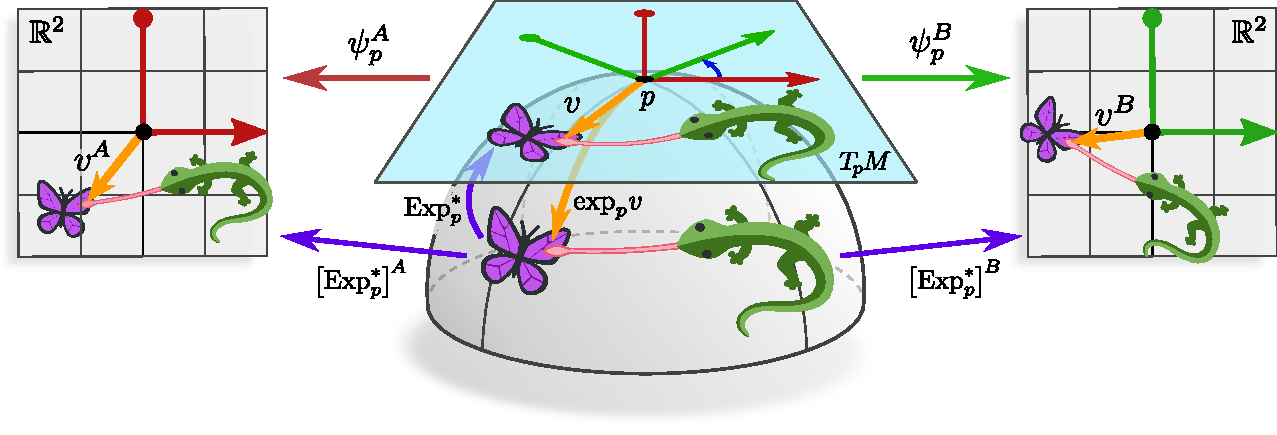
\includegraphics[width=\textwidth]{figures/pullback_field_exp_TpM.pdf}
    \caption{\small
        A feature field $f$ on $M$ and its local representation $\Expspf$ on $\TpM$ via the \emph{transporter pullback} $\Expsp$.
        Just like the usual pullback $\exp_p^*f$ of~$f$ along the exponential map $\exp_p: \TpM \to M$, the transporter pullback assigns feature vectors $f(\exp_p(v))$ to tangent vectors $v\in\TpM$.
        However, as we aim to accumulate the pulled back features by means of a convolution kernel, they need to be given in the same space and be expressed relative to the same gauge at~$p$.
        The transporter pullback therefore additionally applies the ($G$-compatible) parallel transporter along the geodesic from $\exp_p(v)$ to~$p$.
        Via a gauge $\psi_p^X$, the transporter pullback of $f$ on $\TpM$ can be expressed on $\R^d$ as $[\Expspf]^X: \R^d \to \R^c$ -- different choices of reference frames (observers) correspond hereby to different linear deformations of the feature field.
        Kernel field transforms and $\GM$-convolutions compute an output feature~$\fout(p)$ at~$p$ by matching a kernel~$\Kp$ on $\TpM$ with $\Expspf$ (i.e. integrate their product over the tangent space; see Eq.~\eqref{eq:kft_coord_expression}).
        { \\
        \color{gray}
        \scriptsize
            (Lizards and butterflies adapted under the Creative Commons Attribution 4.0 International
            \href{https://github.com/twitter/twemoji/blob/gh-pages/LICENSE-GRAPHICS}{\underline{license}}
            by courtesy of Twitter.)
        }
    }
    \label{fig:pullback_field_exp_TpM}
\end{figure}


We formalize $\Expspf$ by defining it in terms of its coordinate expression relative to some choice of gauge.
To this end, let $\psi_p^A$ be a gauge at $p$, relative to which the transported features will ultimately be expressed and let $\psi_{\exp_p(v)}^{\widetilde{A}}$ be an arbitrary gauge at $\exp_p(v)$, which represents the feature vector at that location by a coefficient vector $f^{\widetilde{A}}(\exp_p(v)) \in \R^c$.
Denote by 
\begin{align}
    \rho \big( g^{A\widetilde{A}}_{p\leftarrow\exp_p\!v} \big)
\end{align}
the $G$-compatible parallel transporter of feature vector coefficients along the geodesic from $\exp_p(v)$ to~$p$.
Then we define the \emph{transporter pullback} in coordinates as%
\begin{align}\label{eq:transporter_pullback_in_coords}
    \big[\mkern-2mu \Expspf \big]^A:\ \R^d \to \R^c,\quad v^A &\mapsto\ \big[\mkern-2mu \Expspf \big]^A (v^A)
        \notag \\[1.5ex]
        & \,:=\ 
        \rho\pig( g^{A\widetilde{A}}_{p \,\leftarrow\, \exp_p (\psi_p^A)^{\shortminus1}(v^A)} \pig) \cdot
        f^{\widetilde{A}} \pig( \exp_p \big(\psi_p^A\big)^{\mkern-2mu-1}(v^A) \pig) \,,
\end{align}
where $v = \big(\psi_p^A\big)^{-1} (v^A) \in \TpM$ is the coordinate free tangent vector referred to by the coefficients $v^A$ via~$\psi_p^A$.
As claimed before, the choice of gauge $\psi_{\exp_p(v)}^{\widetilde{A}}$ at $\exp_p(v)$ is by the coordinate independence of all equations irrelevant and cancels out.
Specifically, one could have used any other gauge $\psi_{\exp_p(v)}^{\widetilde{B}}$ at $\exp_p(v)$, implying gauge transformations
$
    \rho\big( g^{A\widetilde{B}}_{p \,\leftarrow\, \exp_p(v)} \big)
  = \rho\big( g^{A\widetilde{A}}_{p \,\leftarrow\, \exp_p(v)} \big)
    \rho\big( g_{\exp_p(v)}^{\widetilde{B}\widetilde{A}} \big)^{-1}
$
of the transporter by Eq.~\eqref{eq:transporter_gauge_trafo} and
$
    f^{\widetilde{B}} \big( \exp_p(v) \big)
  = \rho\big( g_{\exp_p(v)}^{\widetilde{B}\widetilde{A}} \big)
    f^{\widetilde{A}} \big( \exp_p(v) \big)
$
of the feature vector coefficients by Eq.~\eqref{eq:gauge_trafo_features}, which annihilate when composing both expressions.


The transporter pullback $[\Expspf]^A$ depends, however, still on the gauge at $p$, and therefore transforms under gauge transformations $g_p^{BA}$ at~$p$.
As for any coordinatized function, its transformation law is determined by the gauge transformations on its domain~$\R^d$ and codomain~$\R^c$.
It is therefore given by
\begin{align}\label{eq:trafo_law_transporter_pullback}
    \big[ \Expspf \big]^B\ =\ \rho\big( g_p^{BA} \big) \circ \big[ \Expspf \big]^A \circ \big(g_p^{BA} \big)^{-1} \,,
\end{align}
which is summarized by the following commutative diagram:
\begin{equation}\label{cd:}
\begin{tikzcd}[column sep=70pt, row sep=32pt, font=\normalsize]
    \R^d
        \arrow[d, "g_p^{BA} \cdot\,"']
        \arrow[r, "{\big[\mkern-1mu \Expspf \big]^A}"]
    &
    \R^c
        \arrow[d, "\ \rho\big(g_p^{BA}\big) \cdot"]
    \\
    \R^d
        \arrow[r, "{\big[\mkern-1mu \Expspf \big]^B}"']
    &
    \R^c
\end{tikzcd}
\end{equation}
As visualized in Fig.~\ref{fig:pullback_field_exp_TpM}, $\big[\Expspf\big]^A$ and $\big[\Expspf\big]^B$ should be thought of as the perspective of different local observers (reference frames) on the feature field.


In principle, one could consider alternative constructions for the pullback of feature fields from~$M$ to~$\TpM$.
Our definition of kernel field transforms and $\GM$-convolutions in Sections~\ref{sec:kernel_field_trafos} and~\ref{sec:gauge_conv} below is independent from this particular choice.








\subsubsection{Coordinate independent kernels and kernel field transforms}
\label{sec:kernel_field_trafos}

$\GM$-convolutions are coordinate independent operations which apply the same, shared kernel at each point of the manifold.
To clearly separate the assumptions being made, we first discuss more general \emph{kernel field transforms}, which are coordinate independent operations but drop the requirement of weight sharing.
They are therefore similar to $\GM$-convolutions but apply a potentially different kernel $\Kp$ to each point~$p$ of the manifold.
In order to respect the principle of covariance, the coordinate expressions of those kernels are required to transform in a principled manner, however, the kernels themselves are left unconstrained.


\paragraph{Coordinate independent kernels:}
Since convolutions in deep learning map between fields of feature vectors of dimensionalities $\R^\cin$ and $\R^\cout$, the convolution kernels are ${\cout \mkern-3mu\times\mkern-1.5mu \cin}$ matrix-valued.
Discretized implementations of $d$-dimensional convolutions on Euclidean spaces typically represent such kernels as arrays of shape $(s_1,\dots,s_d, \; c_\text{out},c_\text{in} \mkern1mu)$.
The first $d$~axes represent hereby a spatial grid of $s_1 \times\dots\times s_d$ pixels, each of which is assigned a ${\cout \mkern-3mu\times\mkern-1.5mu \cin}$ matrix, encoded in the last two axes.%
\footnote{
    The actual memory layout depends on the particular deep learning framework in consideration.
}
In the continuous, Euclidean setting, such kernels can be described as maps
\begin{align}\label{eq:conv_kernel_unrestricted}
    K: \R^d \to \R^{\cout\times\cin} \,,
\end{align}
which assign a ${\cout \mkern-3mu\times\mkern-1.5mu \cin}$ matrix to each point of $\R^d$.
As mentioned in the previous Section~\ref{sec:observers_view}, we define $\GM$-convolutions as matching the transporter pullback $\Expspfin$
on the tangent space $\TpM$ with a kernel $\Kp$ on~$\TpM$.
Since the tangent spaces are flat, it is natural to define this matching as in the usual, fully Euclidean setting.
We do therefore define the kernels $\Kp$ via their coordinate expressions, which take the form in Eq.~\eqref{eq:conv_kernel_unrestricted}, that is,
\begin{align}
    \Kp^A: \R^d \to \R^{\cout\times\cin} \,.
\end{align}
Fig.~\ref{fig:kernel_coordinatization} shows a \emph{given} coordinate free kernel on~$\TpM$ and its representations on $\R^d$ relative to different reference frames.%
\footnote{
    We emphasize that we are here assuming a coordinate free kernel $\Kp$ which is \emph{given} on $\TpM$ and consider its coordinate expressions $\Kp^X$ on $\R^d$ relative to reference frames~$X$.
    Convolutional weight sharing will later on pose us with the question of how to \emph{define} a coordinate free kernel $\Kp$ on $\TpM$ given a template kernel $K$ on $\R^d$.
    Appendix~\ref{apx:coord_indep_weight_sharing} elaborates on these two concepts and their relation to the kernel's $G$-steerability.
}


\begin{figure}
    \centering
    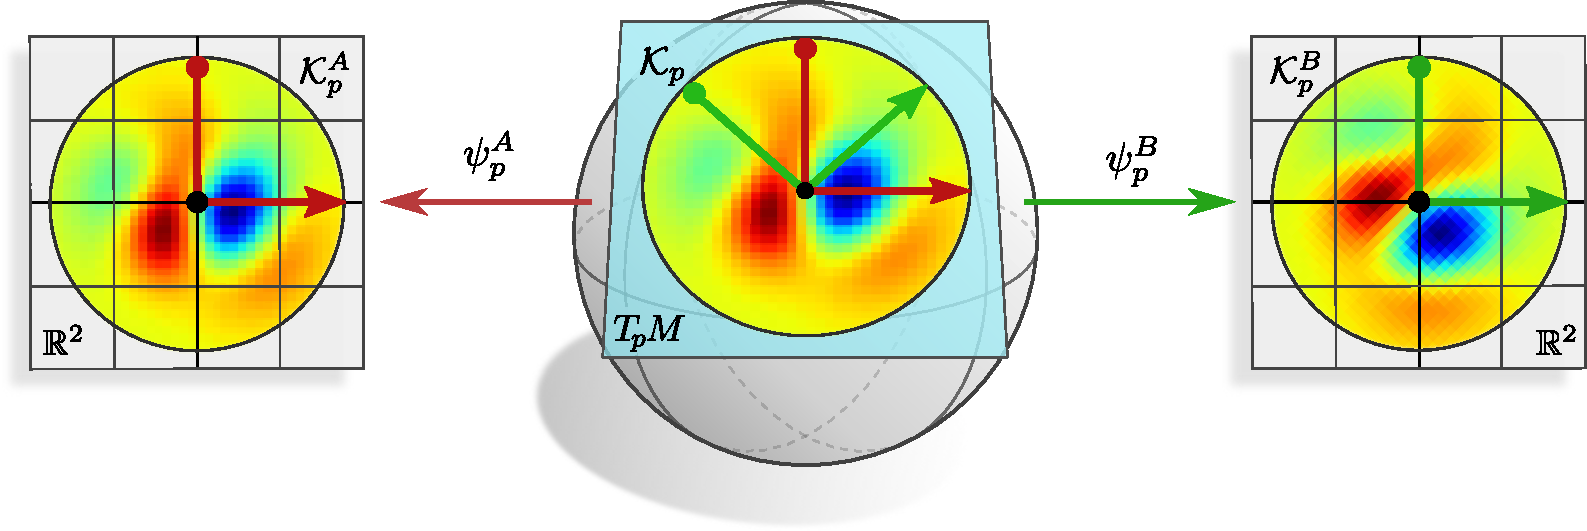
\includegraphics[width=.9\columnwidth]{figures/kernel_coordinatization.pdf}
    \caption{\small
        A coordinate free kernel $\Kp$ on $\TpM$ and its coordinate expressions ${\Kp^X \!: \R^d \to \R^{\cout\times\cin}}$ relative to gauges $\psi_p^X$ (only one of the ${\cout \times \cin}$ kernel channels is shown).
        The gauge transformations that relate different coordinatizations of a kernel follow from the transformation laws of their domain $\R^d$ and codomain $\R^{\cout\times\cin}$.
        They are therefore for any $\mathscr{v} \in \R^d$ given by
        $\Kp^B\big(g_p^{BA} \mathscr{v}\big) = \rhoout\big(g_p^{BA}\big) \:\Kp^A (\mathscr{v})\: \rhoin\big(g_p^{BA}\big)^{-1}$.
        A kernel field $\K$ on $M$ is a smooth assignment of kernels over the tangent spaces (Def.~\ref{dfn:kernel_field_general}).
        \\
        Note that we are here assuming the kernel on $\TpM$ to be given and express it subsequently relative to different gauges on $\R^d$.
        This is conceptually different from the situation depicted in
        Figs.~\ref{fig:satellite}, \ref{fig:intro_kernel_alignment_trivial}, \ref{fig:gauge_trafos_feature_vector} and~\ref{fig:kernel_apx_sharing},
        where we assume a template kernel~$K$ to be given on $\R^d$ and subsequently define $\Kp$ on $\TpM$ via convolutional weight sharing relative to some reference frame.
        In order to preserve coordinate independence during the weight sharing process, the shared kernel needs to be \emph{invariant} (or equivariant) under gauge transformations; see Section~\ref{sec:gauge_conv} and Appendix~\ref{apx:coord_indep_weight_sharing}.
    }
    \label{fig:kernel_coordinatization}
\end{figure}


The transformation law between the coordinate representations $\Kp^A$ and $\Kp^B$ of a kernel $\Kp$ on $\TpM$ follows as usual from the transformation laws of their domain and codomain.
On the domain $\R^d$ the transformation law is given by $g_p^{BA}$, while the transformation law of $\R^{\cout\times\cin}$ is, as in Eq.~\eqref{eq:linear_op_trafo_law}, given by a simultaneous left multiplication with $\rhoout\big(g_p^{BA}\big)$ and right multiplication with $\rhoin\big(g_p^{BA}\big)^{-1}$.
The two coordinatizations of the kernel $\Kp$ relate thus for any $\mathscr{v} \in \R^d$ by
\begin{align}\label{eq:kernel_trafo_law}
    \Kp^B\big(g_p^{BA} \mathscr{v}\big)\ =\ 
    \rhoout\big(g_p^{BA}\big) \cdot\mkern1mu 
    \Kp^A (\mathscr{v})
    \mkern1mu\cdot \rhoin\big(g_p^{BA}\big)^{-1} \,,
\end{align}
which is visualized by the following commutative diagram:
\begin{equation}\label{cd:kernel_trafo_law}
\qquad
\begin{tikzcd}[column sep=70pt, row sep=32pt, font=\normalsize]
    \R^d
        \arrow[d, "g_p^{BA} \cdot\,"']
        \arrow[r, "\Kp^A"]
    &
    \R^{\cout\times\cin}
        \arrow[d, "\ \rhoout\big(g_p^{BA}\big) \; \scalebox{1.1}{$[\,\cdot\,]$} \; \rhoin\big(g_p^{BA}\big)^{-1}"]
    \\
    \R^d
        \arrow[r, "\Kp^B"']
    &
    \R^{\cout\times\cin}
\end{tikzcd}
\end{equation}
As in the examples from Section~\ref{sec:pointwise_operations}, the principle of covariance only requires a consistent transformation behavior between different kernel coordinatizations but does not lead to a constraint on the kernel itself.
One might therefore parameterize the kernels $\Kp$ for any $p\in M$ and an arbitrary gauge at $p$ by some unrestricted, matrix-valued kernel.
We denote smooth fields of such kernels as kernel fields, which play a major role in our analysis of the isometry equivariance of $\GM$-convolutions in Section~\ref{sec:isometry_intro}.



\paragraph{Coordinate independent kernel field transforms:}
Given a smooth kernel field $\K$, we can define \emph{kernel field transforms}, which are similar to convolutions but differ in that they might apply a different kernel at each spatial position.
They compute a field of output feature vectors $\fout(p)$ by
integrating the product of the corresponding kernel $\Kp$ and transporter pullback $\Expspfin$ of $\fin$ over $\TpM$, that~is,
\begin{align}\label{eq:kft_coord_free}
    \fout(p)\ =\ 
    \int_{\TpM}
    \Kp(v) \,
    \Expspfin(v) \;
    dv \,.
\end{align}
To express this coordinate free definition in terms of coordinates, one has to replace all quantities by their coordinate expressions and to pull the integration via the chosen gauge from $\TpM$ to $\R^d$.
As described in Appendix~\ref{apx:tangent_integral}, the appropriate (gauge invariant) Riemannian volume element is for a gauge $\psi_p^A$ given by
\begin{align}
    \sqrt{|\eta_p^A|} \,\ dv^A ,
\end{align}
where the factor $\sqrt{|\eta_p^A|}$, defined in Eq.~\eqref{eq:volume_element_def}, is the (positive) volume spanned by the reference frame $[e_i^A]_{i=1}^d$ at~$p$.
The coordinate expression of the kernel field transform thus reads
\begin{align}\label{eq:kft_coord_expression}
    \fout^A(p)
    \ =&\ 
        \int_{\R^d}
        \Kp^A(v^A) \ 
        \big[\mkern-2mu \Expspfin\big]^A \mkern-1mu(v^A) \ 
        \sqrt{|\eta_p^A|}\ dv^A
    \,.
\end{align}

The coordinate independence of the kernel field transform is asserted by expressing it relative to an alternative gauge $\psi_p^B$ and showing that the resulting output field transforms as expected, which is indeed the case:
\begin{align}\label{eq:kft_coordinate_independence}
    \fout^B(p)\ 
    \overset{(1)}{=}&\ 
        \int_{\R^d}
        \Kp^B(v^B) \ 
        \big[\mkern-2mu \Expspfin\big]^B \mkern-2mu(v^B) \,\ 
        \sqrt{|\eta_p^B|}\ dv^B
    \notag \\ 
    \overset{(2)}{=}&\ 
        \int_{\R^d}
        \Big[ \rhoout\big(g_p^{BA}\big)\, \Kp^A\pig(\! \big(g_p^{BA}\big)^{-1} v^B \big)\!\pig)\, \rhoin\big(g_p^{BA}\big)^{-1} \Big] \,\ 
        \big[\mkern-1mu \Expspfin\big]^B \mkern-2mu(v^B) \,\ 
        \sqrt{|\eta_p^B|}\ dv^B
    \notag \\ 
    \overset{(3)}{=}&\ \ 
        \rhoout\big(g_p^{BA}\big)
        \int_{\R^d}
        \Kp^A(v^A) \,\ 
        \Big[ \rhoin\big(g_p^{BA}\big)^{-1} \big[\mkern-1mu \Expspfin\big]^B \mkern-2mu \big( g_p^{BA} v^A\big) \Big] \ 
        \sqrt{|\eta_p^A|}\ dv^A
    \notag \\ 
    \overset{(4)}{=}&\ \ 
        \rhoout\big(g_p^{BA}\big)
        \int_{\R^d}
        \Kp^A(v^A) \,\ 
        \big[\mkern-1mu \Expspfin\big]^A \mkern-1mu (v^A) \ 
        \sqrt{|\eta_p^A|}\ dv^A
    \notag \\ 
    \overset{(5)}{=}&\ \ 
    \rhoout\big(g_p^{BA}\big) \, \fout^A(p)
\end{align}
Here we used the definition of kernel field transforms and the transformation law of kernels (Eq.~\eqref{eq:kernel_trafo_law}) in the first two steps.
The third step follows by pulling $\rhoout$ out of the integral and substituting $v^B$ with $v^A = \big(g_p^{BA}\big)^{-1} v^B$, using that the volume element $\sqrt{|\eta_p^B|}\ dv^B = \sqrt{|\eta_p^A|}\ dv^A$ is by design gauge invariant.
The last two steps follow then by identifying the transformation law of the transporter pullback of the feature field in Eq.~\eqref{eq:trafo_law_transporter_pullback} and the definition of the kernel field transform in gauge $\psi_p^A$.
Note that the coordinate independence of the kernel field transform affirms the correctness of the kernel transformation law in Eq.~\eqref{eq:kernel_trafo_law}.

A kernel field transform is only well defined if the integrals over the tangent spaces converge, which is more rigorously discussed in Section~\ref{sec:global_conv} and Appendix~\ref{apx:smoothness_kernel_field_trafo}.
Theorem~\ref{thm:existence_kernel_field_trafo_compact_kernels} proves that a compact support of the kernels $\Kp$ is sufficient to guarantee this well-definedness.
It further proves that kernel field transforms that are based on smooth kernel fields will map smooth input feature fields to smooth output feature fields.












\subsubsection{\textit{GM}-convolutions and \textit{G}-steerable kernels}
\label{sec:gauge_conv}

The freedom of kernel field transforms to apply a different kernel at each location does not allow them to generalize learned inference over different locations and thus makes them data inefficient.
One does therefore typically consider convolutions, which can be seen as those specific kernel field transforms that are based on convolutional kernel fields, i.e. kernel fields that are parameterized by a single, shared template kernel.
As before, a coordinate independent weight sharing requires the template kernels to be gauge equivariant ($G$-steerable).
This gauge equivariance of the template kernels implies that patterns which appear in different, $G$-related geometric poses are guaranteed to evoke the same response up to a corresponding transformation of the feature vector via $\rhoout$.


\paragraph{Convolutional weight sharing:}
Let $K: \R^d \to \R^{\cout\times\cin}$ be a template kernel to be shared over all tangent spaces.
In order to not prefer any particular gauge -- which would contradict our requirement for coordinate independence -- we are forced to share the kernel with coordinatizations in all gauges simultaneously.
Naively, this seems to suggest to share the template kernel by setting $\Kp^X = K$ for any point $p\in M$ and any gauge $\psi_p^X$ at~$p$.
While such a definition of kernel sharing seems reasonable, it does not follow our principle of sharing local template functions in a strict sense:
instead of directly sharing the kernel, it is important to share the \emph{whole} local operation -- which is here the whole 
integral transform in Eq.~\eqref{eq:kft_coord_expression}.
Since this operation is parameterized in terms of the kernel field $\K$, this leads indirectly to a sharing of the template kernel, however, with a slightly different result as the naive sharing considered above.

To find the correct definition of $\GM$-convolutional kernel fields according to our principle of sharing local template functions, we first need to identify these local operations.
We do this by abstracting kernel field transforms (in coordinates) as a collection of local integral operators of the form
\begin{align}\label{eq:local_integral_operator_general}
    \mathscr{I}_{\K,p}^A:\ 
    C^\infty \big(\R^d, \R^c\big) \to \R^c, \quad
    F \,\mapsto \int_{\R^d} \Kp^A(\mathscr{v})\, F(\mathscr{v})\, \sqrt{|\eta_p^A|}\ d\mathscr{v} \,,
\end{align}
where $C^\infty \big(\R^d, \R^c\big)$ denotes the space of smooth maps from $\R^d$ to $\R^c$.
In our application, these smooth maps are just the local feature field representations $[\Expspf]^A: \R^d \to \R^c$ as seen from the tangent spaces at~$p$, which are by the kernel field transform mapped to an output feature vector $\fout^A(p) = \mathscr{I}_{\K,p}^A \big([\Expspf]^A\big)$ at~$p$.
Given our template kernel $K: \R^d \to \R^{\cout\times\cin}$, we define a corresponding integral operator template
\begin{align}\label{eq:local_integral_operator_template}
    \mathfrak{I}_K:\ 
    C^\infty \big(\R^d, \R^c\big) \to \R^c, \quad
    F \,\mapsto \int_{\R^d} K(\mathscr{v})\, F(\mathscr{v})\ d\mathscr{v} \,,
\end{align}
which multiplies the local field representation $F$ with the template kernel $K$ and then integrates their product.
Note that $\mathfrak{I}_K$ is as a template function necessarily agnostic to specific choices of gauges and does therefore not involve a frame volume factor.
A $\GM$-coordinate independent convolutional weight sharing scheme is imposed by demanding that this template functional agrees with all the individual integral operators at any point and in any gauge, that is,
\begin{align}\label{eq:weight_sharing_integral_operator}
    \mkern28mu
    \mathscr{I}_{\K,p}^X = \mathfrak{I}_K
    \quad \textup{for \emph{any} gauge}\ \ \big(U^X,\psi^X) \in \mathscr{A}^G\ \ \textup{with}\ \ p\in U^X \,,
\end{align}
where $\mathscr{A}^G$ is the (maximal) $G$-atlas corresponding to the considered $G$-structure; see Eq.~\eqref{eq:G_atlas_dfn}.
This is equivalent to directly sharing the local template kernel according to
\begin{align}\label{eq:weight_sharing_kernel}
    \Kp^X = \frac{K}{\sqrt{|\eta_p^X|}\,}
    \quad \textup{for \emph{any} gauge}\ \ \big(U^X,\psi^X) \in \mathscr{A}^G\ \ \textup{with}\ \ p\in U^X \,,
\end{align}
where the normalization factor reduces the ``kernel density'' by the reference frame volume $\sqrt{|\eta_p^X|}$.
As discussed below, this normalization is important for the equivariance under non-volume-preserving symmetry groups


We denote kernel fields which are parameterized by a shared kernel $K$ according to Eq.~\eqref{eq:weight_sharing_kernel} as $\GM$-\emph{convolutional kernel fields}.
The simultaneous requirement for weight sharing and coordinate independence leads to an equivariance constraint on the template kernels.
To derive this constraint, insert the kernel sharing in Eq.~\eqref{eq:weight_sharing_kernel} into the kernel transformation law in Eq.~\eqref{eq:kernel_trafo_law}, which results in
\begin{align}
    \frac{1}{\sqrt{|\eta_p^B|\,}}\ K\big(g_p^{BA} \mathscr{v}\big)
    \ =\ 
    \frac{1}{\sqrt{|\eta_p^A|\,}}\ 
    \rhoout\big(g_p^{BA}\big) \cdot\mkern1mu 
    K(\mathscr{v})
    \mkern1mu\cdot \rhoin\big(g_p^{BA}\big)^{-1} \,.
\end{align}
Since the volumes of different reference frames are related by
$\sqrt{|\eta_p^A|} = \big|\mkern-2mu \det(g_p^{BA})\big|\, \sqrt{|\eta_p^B|}$
and since the transformation law needs to hold for arbitrary $G$-related gauges, this implies the \emph{$G$-steerability} constraint%
\footnote{
    In contrast to prior work~\cite{3d_steerableCNNs,Weiler2019_E2CNN,gaugeIco2019,kicanaoglu2019gaugeSphere,deHaan2020meshCNNs}, this constraint contains the factor $\detg$.
    It did not appear in these works since they all considered (subgroups of) orthonormal structure groups $\O{d}$, for which the determinant factor vanishes.
}
\begin{align}\label{eq:kernel_constraint}
    K(g\mkern1.5mu \mathscr{v})\ = \ \frac{1}{\detg}\, \rhoout(g) \cdot K(\mathscr{v}) \cdot \rhoin(g)^{-1}
    \qquad \forall\ \ \mathscr{v} \in \R^d,\ \ g\in G \,.
\end{align}
on template kernels.
As proven by~\citet{lang2020WignerEckart}, this constraint requires template kernels to be \emph{representation operators}~\cite{jeevanjee2011reprOp} (generalizations of e.g. spherical tensor operators in quantum mechanics).
Diagrammatically, a $G$-steerable kernels $K$ is required to satisfy the commutativity of
\begin{equation}\label{cd:kernel_steerability}
\qquad\qquad
\begin{tikzcd}[column sep=70pt, row sep=35pt, font=\normalsize]
    \R^d
        \arrow[d, "g\mkern2mu \cdot\,"']
        \arrow[r, "K"]
    &
    \R^{\cout\times\cin}
        \arrow[d, "\ \scalebox{.96}{$\displaystyle \frac{1}{\detg}$}\, \rhoout(g) \; \scalebox{1.1}{$[\,\cdot\,]$} \; \rhoin(g)^{-1}"]
    \\
    \R^d
        \arrow[r, "K"']
    &
    \R^{\cout\times\cin}
\end{tikzcd}
\end{equation}
for any $g\in G$.
Note that the inverse determinant factor $\detg$ in the kernel's transformation law makes it transform like a \emph{matrix-valued $-1$-density}; see Table~\ref{tab:density_factors} for more details.
Intuitively, $G$-steerable kernels are exactly those kernels that can be shared relative to arbitrary $G$-related reference frames without that the particular choice of gauge would influence the result.%
\footnote{
    The $G$-steerability constraint can be rewritten as
    ${K(\mathscr{v}) = \detg^{\minus1} \rhoout(g) \mkern-1mu\cdot\mkern-1.5mu K(g^{\minus1}\mathscr{v}) \mkern-1mu\cdot\mkern-1.5mu \rhoin(g)^{\minus1}}$
    $\mkern8mu \forall\ \mathscr{v} \in \R^d,\ g\in G$,
    which emphasizes that $G$-steerable kernels are the \emph{invariants} under the gauge action on the right-hand-side.
    Being invariant under gauge transformations, a $G$-steerable kernel leads to the same coordinate free kernel $\Kp$ at $p$ when being shared relative to any reference frame in~$\GpM$.
}
The ambiguity of kernel alignments -- which motivated this work in the first place -- is thus resolved by additional weight sharing over all the equivalent reference frames (all gauges) in the considered $G$-structure~$\GM$.


\begin{table}
    \centering
    \setlength\aboverulesep{0pt}
    \setlength\belowrulesep{0pt}
    \renewcommand{\arraystretch}{1.8}
    \setlength{\tabcolsep}{2.4ex}
    \scalebox{.95}{
    \begin{tabular}{l|ccccccc}
        object     & $\Kp^X$ & $K$  & $\big[\mkern-2mu\Expspf\big]^{\mkern-2muX}\mkern-2mu$ and $F$ & $\sqrt{|\eta^X|}$ & $dv^X\!$ and $d\mathscr{v}$ \\
       \midrule
       density $s$ & $0$     & $-1$ & $0$                                                           & $-1$              & $1$
    \end{tabular}
    }
    \vspace*{2ex}
    \caption{
        An overview of the density exponents $s$ of different objects involved in general kernel field transforms and $\GM$-convolutions.
        The coordinate expression of an $s$-density transforms with a factor of $\detg^s$ when the coordinates are transformed via $g\in G$.
        A general matrix-valued kernel $\Kp^X$ is according to Eq.~\eqref{eq:kernel_trafo_law} a $0$-density.
        The same holds for feature fields and their pullbacks, whose transformation laws are given in Eqs.~\eqref{eq:gauge_trafo_features} and~\eqref{eq:trafo_law_transporter_pullback}.
        The whole integrand $\Kp^X(v^X) [\Expspf]^{\mkern-1muX}(v^X) \sqrt{|\eta^X|}\, dv^X$ of a general kernel field transforms in Eq.~\eqref{eq:kft_coord_expression} is seen to be a $0$-density as well -- note that this is necessary for its coordinate independence as demonstrated in Eq.~\eqref{eq:kft_coordinate_independence}.
        As the integral operator template $\mathfrak{I}_K$ in Eq.~\eqref{eq:local_integral_operator_template} is agnostic of any choice of gauge, it does not involve the frame volume factor $\sqrt{|\eta^X|}$.
        Since it should nonetheless behave like the integral operators $\mathscr{I}_{\K,p}^X$ underlying kernel field transforms, the whole integrand $K(\mathscr{v}) F(\mathscr{v})\, d\mathscr{v}$ of $\mathfrak{I}_K(F)$ is required to be a $0$-density.
        This necessitates the shared template kernels $K$ themselves to transform like $-1$-densities, which is reflected in the $G$-steerability constraint in Eq.~\eqref{eq:kernel_constraint}.
        Note that this transformation law of template kernels is strictly necessary for the local $G$-equivariance of $\GM$-convolutions if the output features should transform like densities of weight~$0$; see Eq.~\eqref{eq:active_local_gauge_trafo}.
        For an alternative perspective, we point the interested reader to Corollary~1 in~\cite{bekkers2020bspline}, where the determinant factor is derived from Haar measures on Lie groups.
    }
    \label{tab:density_factors}
\end{table}

Before coming to $\GM$-convolutions, we comment on the space of $G$-steerable kernels.
Note that the set
\begin{align}\label{eq:unconstrained_kernel_space}
    \mathscr{K}\ :=\ \pig\{ K\!: \R^d \to \R^{\cout\times\cin} \pig\} \,.
\end{align}
of general, i.e. not necessarily equivariant kernels forms a vector space when being equipped with the standard summation and scalar multiplication on $\R^{\cout\times\cin}$.
Since the $G$-steerability constraint in Eq.~\eqref{eq:kernel_constraint} is linear, it restricts the kernel space to a \emph{linear subspace}
\begin{align}\label{eq:G-steerable_kernel_space}
    \KG\, :=\ \Big\{ K\!: \R^d \to \R^{\cout\times\cin} \,\Big|\,
    K(g\mkern1mu \mathscr{v}) = \frac{1}{\detg}\, \rhoout(g) \mkern-1.5mu\cdot\mkern-1.5mu K(\mathscr{v}) \mkern-1.5mu\cdot\mkern-1.5mu \rhoin(g)^{-1} \ \ \ \forall\,\ \mathscr{v}\in \R^d,\,\ g\in G \Big\} \,.
\end{align}
It is therefore possible to solve for a basis of $G$-steerable kernels, in terms of which the $\GM$-convolution can be parameterized.
While this space is in theory usually infinite-dimensional, it is in practice often being discretized, such that one ends up with a finite basis $\{K_1,\dots,K_N\}$ of $G$-steerable kernels.
A~set $\{w_1,\dots,w_N\}$ of real-valued weights $w_i\in\R$, which are optimized during the training process, then parameterize the convolution with $K = \sum_{i=1}^N w_i K_i$.
Note that the reduced dimensionality of the (sub)space of $G$-steerable kernels implies an improved parameter efficiency in comparison to conventional convolutions.


Section~\ref{sec:mobius_kernel_spaces} discusses exemplary analytical solutions of reflection equivariant kernels spaces for different group representations of the reflection group~$\Flip$.
The resulting kernels, which are characterized by different types of reflectional symmetries, are visualized in Table~\ref{tab:reflection_steerable_kernels}.


Further examples can be found in the literature on steerable CNNs:
an analytical solution of the kernel space constraint for the special orthogonal structure group $\SO3$ in three dimensions and its irreducible representations was presented by~\citet{3d_steerableCNNs}.
\citet{Weiler2019_E2CNN} generalized this approach to cover arbitrary group representations and solved the kernel space constraint for any representation of $\O2$ and all of its subgroups $G\leq\O2$
-- an implementation is available at \url{https://quva-lab.github.io/e2cnn/api/e2cnn.kernels.html}.
For finite structure groups the constraint might alternatively be solved numerically as explained by~\citet{Cohen2017-STEER}.
A more general solution strategy, applying to arbitrary compact structure groups~$G$ (and thus all above mentioned cases), was proposed by~\citet{lang2020WignerEckart}.
This solution generalizes the classical \emph{Wigner-Eckart} theorem~\cite{agrawalla1980WignerEckart,jeevanjee2011reprOp,wigner1931gruppentheorie,wigner1993matrices} to a Wigner-Eckart theorem for $G$-steerable kernels, which expresses the kernels in terms of harmonic basis functions, Clebsch-Gordan coefficients and endomorphisms of the representations (generalized reduced matrix elements).
We refer to~\cite{lang2020WignerEckart} for a more detailed overview on prior and related work on steerable kernels.












\paragraph{\textit{GM}-coordinate independent convolutions:}

Given a $G$-steerable template kernel $K\in\KG$, the $\GM$-convolution~$K\star$ with this kernel is defined as the kernel field transform with the corresponding $\GM$-convolutional kernel field, satisfying $\Kp^X = K / \sqrt{|\eta^X|}$ for any point $p\in M$ and any gauge $\psi_p^X$.
By inserting the $\GM$-convolutional kernel field into Eq.~\eqref{eq:kft_coord_expression}, i.e. the kernel field transform, the coordinate expression of the $\GM$-convolution boils down to
\begin{align}\label{eq:gauge_conv_coord_expression}
    \fout^A(p)
    \ =\ 
    \big[ K \star \fin \big]^A(p)
    \ :=&\,\ 
        \int_{\R^d} \!
        K(\mathscr{v}) \,
        \big[\mkern-2mu \Expspfin\big]^{\mkern-2mu A} \mkern-1mu(\mathscr{v})
        \; d\mathscr{v}
    \ \ =\,\ \mathfrak{I}_K \big( [\Expspfin]^A \big)
    \,.
\end{align}
It is thus simply given by matching the transporter pullback $[\Expspfin]^A$ of the feature field in an \emph{arbitrarily chosen gauge} $\psi_p^A$ with the \emph{gauge independent} convolution kernel~$K$.
$\GM$-coordinate independent convolutions are therefore easily implemented by
1) choosing arbitrary reference frames,
2) pulling (and transporting) the feature fields back to the tangent space coordinatizations and
3) contracting them there with a (trainable) $G$-steerable kernel.

$\GM$-convolutions exhibit multiple related symmetry properties:
\begin{itemize}[leftmargin=13em]
    \item[\it coordinate independence:]
        As specific instances of kernel field transforms, $\GM$-convolutions are (passively) coordinate independent, i.e. Eq.~\eqref{eq:kft_coordinate_independence} applies to them.
    \item[\it global isometry equivariance:]
        They are equivariant under the \emph{active}, \emph{global} action of $G$-structure preserving isometries in $\IsomGM$ on feature fields.
        Sections~\ref{sec:gauge_conv_isom_equiv} and specifically~\ref{sec:isometry_intro} discuss this property in detail.
    \item[\it local $G$-equivariance:]
        The integral operator template $\mathfrak{I}_K$ is by the $G$-steerability of~$K$ itself $G$-equivariant.
        Any $G$-transformation of a local feature field representation on $\R^d$ will therefore result in a corresponding transformation of the resulting feature vector; see Fig.~\ref{fig:active_TpM_equivariance}.
        Independent $G$-transformations of patterns that are centered at different points $p_i\in M$ will therefore lead to independent output feature transformations at these points (this holds \emph{only} at these points and requires compactly supported kernels whose entire \emph{field of view} transforms according to the $G$-transformation).
\end{itemize}


\begin{figure}
    \centering
    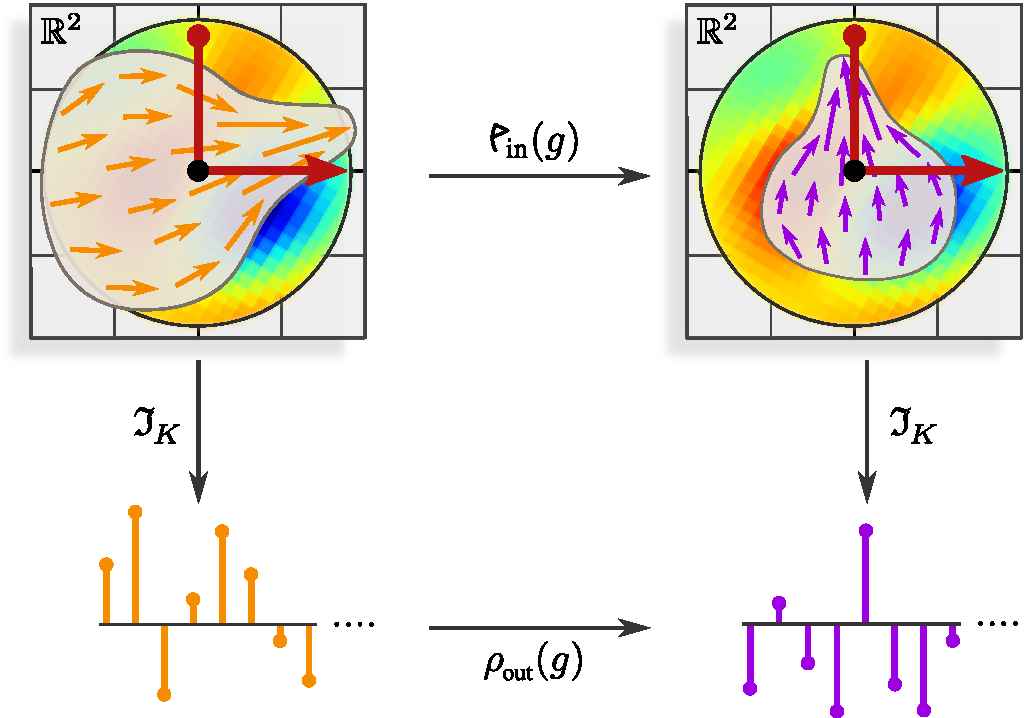
\includegraphics[width=.65\columnwidth]{figures/active_TpM_equivariance.pdf}
    \vspace*{1ex}
    \caption{\small
        Local $G$-equivariance of the shared integral operator template $\mathfrak{I}_K$ underlying a $\GM$-convolution~$K\star$.
        An active $G$-transformation $\textphnc{b}_{\mkern-5mu\textup{in}}(g)$ of a local field representation on $\R^d$ moves feature vectors from $g^{-1}\mathscr{v}$ to~$\mathscr{v}$ and transforms them additionally via $\rhoin(g)$.
        While the former moves features spatially, the latter transforms their numerical coefficients (visualized as rotation and scaling of the individual (tangent) vectors in the figure).
        The application of $\mathfrak{I}_K$ to both inputs results in different output feature vectors.
        However, by the $G$-equivariance of $\mathfrak{I}_K$, the responses are guaranteed to be related by $\rhoout(g)$; see Eq.~\eqref{eq:active_local_gauge_trafo}.
        An active $G$-transformation of an input field therefore results in a corresponding active $G$-transformation of the output feature vector.
        Note that the $G$-equivariance of $\mathfrak{I}_K$ is a direct consequence of the $G$-steerability of $K$.
        \\\protect\rule{0ex}{0.5ex}
        }
    \label{fig:active_TpM_equivariance}
\end{figure}


To make the last point precise, we define active $G$-transformations of local feature field representations in $C^\infty(\R^d,\R^c)$ as%
\footnote{
    ${\textphnc{b} = \Res_G^{\R^d\mkern-1mu\rtimes G}\Ind_G^{\R^d\mkern-1mu\rtimes G}\!\rho}$ is formally given by the induction of the $G$-representation $\rho$ to a ${(\R^d\mkern-4mu\rtimes\mkern-2muG)}$-representation ${\Ind_G^{\R^d\mkern-1mu\rtimes G}\!\rho}$, followed by a restriction back to $G$.
    An intuitive explanation of induced and restricted representations can be found in Appendix~B of~\cite{Weiler2019_E2CNN} while \cite{gallier2019harmonicRepr} treats the topic more formally.
}
\begin{align}\label{eq:local_field_G_trafo}
    \textphnc{b}_{\mkern-5mu\textup{in}}:\ 
    G \times C^\infty(\R^d,\R^c) \to C^\infty(\R^d,\R^c) \,, \quad
    F \,\mapsto\, \textphnc{b}_{\mkern-5mu\textup{in}}(g)F \,:=\, \rhoin(g) \circ F \circ g^{-1} \,,
\end{align}
where we assume $F$ to be of type $\rhoin$.
Intuitively, $\textphnc{b}_{\mkern-5mu\textup{in}}$ acts on fields $F$ by actively moving feature vectors $F(g^{-1}\mathscr{v}) \in \R^c$ from $g^{-1}\mathscr{v}$ to $\mathscr{v}$, thereby transforming them with $\rhoin(g)$
-- this is the ``usual'' definition of active transformations of feature fields~$F$ on Euclidean spaces~$\R^d$.
The claimed $G$-equivariance of $\mathfrak{I}_K$ is easily seen by applying it to a transformed input, followed by a substitution and making use of the $G$-steerability of~$K$:
\begin{alignat}{3}\label{eq:active_local_gauge_trafo}
\qquad
    \mathfrak{I}_K \big( \textphnc{b}_{\mkern-5mu\textup{in}}(g) F \big)
    \ =&\ \mathfrak{I}_K \big( \rhoin(g) \circ F \circ g^{-1} \big)
        \qquad\quad && \big( \text{\small def. of $\textphnc{b}_{\mkern-5mu\textup{in}}$, Eq.~\eqref{eq:local_field_G_trafo} } \big) \notag\\
    \ =&\ \int_{\R^d} K(\mathscr{v})\; \rhoin(g)\, F\big(g^{-1}\mathscr{v})\ d\mathscr{v}
        \qquad\quad && \big( \text{\small def. of $\mathfrak{I}_K$, Eq.~\eqref{eq:local_integral_operator_template} } \big) \notag\\
    \ =&\ \int_{\R^d} K(g\mkern1mu\tilde{\mathscr{v}})\; \rhoin(g)\, F\big(\tilde{\mathscr{v}})\; \detg \ d\tilde{\mathscr{v}}
        \qquad\quad && \big( \text{\small substitution of $\tilde{\mathscr{v}} = g^{-1} \mathscr{v}$ } \big) \notag\\
    \ =&\ \int_{\R^d} \rhoout(g)\, K(\tilde{\mathscr{v}})\; F\big(\tilde{\mathscr{v}})\ d\tilde{\mathscr{v}}
        \qquad\quad && \big( \text{\small $G$-steerability of $K$, Eq.~\eqref{eq:kernel_constraint} } \big) \notag\\
    \ =&\ \rhoout(g)\; \mathfrak{I}_K(F)
        \qquad\quad && \big( \text{\small def. of $\mathfrak{I}_K$, Eq.~\eqref{eq:local_integral_operator_template} } \big)
\end{alignat}
An active transformation of a local feature field representation $F$ on some tangent space coordinatization by~$\textphnc{b}_{\mkern-5mu\textup{in}}(g)$ is therefore guaranteed to lead to a transformation of the resulting output feature vector by~$\rhoout(g)$.
In other words, features which appear in different $G$-related geometric poses will evoke the same response up to a transformation via~$\rhoout$.
In terms of a commutative diagram, this is concisely summarized as:
\begin{equation}\label{cd:}
\begin{tikzcd}[column sep=56pt, row sep=34pt, font=\normalsize]
    C^\infty(\R^d,\R^{\cin})
        \arrow[d, "\mathfrak{I}_K\,"']
        \arrow[r, "\textphnc{b}_{\mkern-5mu\textup{in}}(g)"]
    &
    C^\infty(\R^d,\R^{\cin})
        \arrow[d, "\ \mathfrak{I}_K"]
    \\
    \R^{\cout}
        \arrow[r, "\rhoout(g)"']
    &
    \R^{\cout}
\end{tikzcd}
\end{equation}
Fig.~\ref{fig:active_TpM_equivariance} gives a visual interpretation of this equivariance property of $\mathfrak{I}_K$.


Note that the equivariance under local $G$-transformations in Eq.~\eqref{eq:active_local_gauge_trafo} requires the $G$-steerability constraint exactly as it is in Eq.~\eqref{eq:kernel_constraint}, that is, in particular, \emph{with} the determinant factor $\detg^{-1}$ which makes the kernel transform like a $-1$-density.
This factor is traced back to our definition of convolutional weight sharing in Eq.~\eqref{eq:weight_sharing_kernel} \emph{with} the normalization by the reference frame volumes $\sqrt{|\eta_p^X|}$.
The naive weight sharing mentioned in the beginning of this section would therefore not have lead to the desired transformation behavior.
In other words: both the naive and the normalized version of the kernel sharing are coordinate independent and behave therefore both consistently under passive gauge transformations -- in particular such which change the frame volume.
However, in the case of the naive kernel sharing, this is taken care of by the invariance of the Riemannian volume element $\sqrt{|\eta_p^A|}\ dv^A = \sqrt{|\eta_p^B|}\ dv^B$.
By \emph{canceling} this factor in the normalized weight sharing, the consistency of the transformation behavior is not guaranteed by the integration measure itself anymore -- which requires the $G$-steerable kernels themselves to explain volume changes via the determinant factor.
Only the latter generalizes to active transformations, where only the feature field is transformed, while the integration measure stays invariant.


As our definition of $\GM$-convolutions allows for arbitrary Riemannian manifolds, G-structures and field types, it is quite general and covers a wide range of related work.
We substantiate this claim in Part~\ref{part:literature_review}, where we explain many CNNs on Euclidean affine spaces $\Euc_d$, the sphere $S^2$ and general manifolds or meshes as specific instantiations of Eq.~\eqref{eq:gauge_conv_coord_expression}.
For an overview and a classification of these models, we refer to Table~\ref{tab:network_instantiations}.
